\documentclass[12pt]{article} 
\usepackage{longtable}
\usepackage{makecell}
\usepackage{float}
\usepackage{graphicx}
\usepackage{bm}
\usepackage{placeins}
\usepackage{booktabs}
\usepackage{gensymb}
\usepackage{subcaption}
\usepackage{amssymb}
\usepackage{indentfirst}
\usepackage{threeparttable} 
\usepackage{multirow}
\usepackage{tabularx}
\usepackage{aligned-overset}
\usepackage[slantfont,boldfont]{xeCJK}
\usepackage{fontspec}
\renewcommand{\arraystretch}{1.5}
% \usepackage[paperwidth=21cm,paperheight=29.7cm]{geometry}
\usepackage[a4paper,margin=2cm]{geometry}
\setCJKmainfont{SimSun}
\setmainfont{SimSun}
\setsansfont{SimSun}
% 设置正文字体为四号（12pt）
% \renewcommand{\CJKmainfont}{SimSun}
\renewcommand{\CJKfamilydefault}{\CJKrmdefault}
\renewcommand{\normalsize}{\fontsize{12pt}{18pt}\selectfont}
\normalsize

\title{RC、RL及RLC串联电路的暂态过程实验报告}
\author{2411545 邱凯锐}
\date{2025.12.15}

\begin{document}
\maketitle
\section{实验目的}
1. 研究 RC、RL、RLC 传输电路的暂态过程。

2. 了解时间常数的物理意义，学会用示波器测量时间常数 $\tau$ 及电容、电感值。

\section{实验原理}
\subsection{RC电路的暂态过程}
\begin{figure}[H]
    \centering
    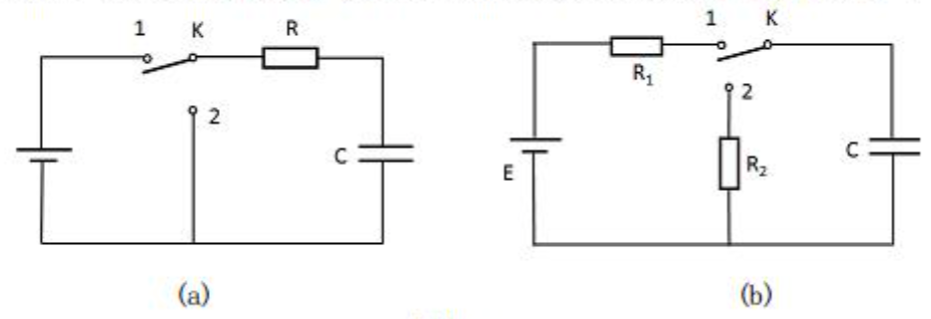
\includegraphics[width=0.7\textwidth]{fig1.png}
    \caption{}
\end{figure}
由电阻 $R$、电容 $C$ 串联的电路，如 Figure 1 所示。
对于 Figure 1(a)，当开关 $K$ 置“1”时，直流电压 $E$ 通过 $R$ 对电容 $C$ 充电。
充电完毕（$u_C=E$），再将 $K$ 由“1”置“2”，电容 $C$ 将通过电阻 $R$ 放电。
充、放电过程均为暂态过程。在暂态过程中电容上的电压 $u_C$ 和电阻上的电压 $u_R$ 随时间 $t$ 的变化规律为：

充电过程
\begin{equation}
    \begin{cases}
        u_C=E(1-e^{-t/\tau})\\
        u_R=Ee^{-t/\tau}
    \end{cases}
\end{equation}

放电过程
\begin{equation}
    \begin{cases}
        u_C=Ee^{-t/\tau}\\
        u_R=-Ee^{-t/\tau}
    \end{cases}
\end{equation}

式中 $\tau=RC$，称为该电路的时间常数，它决定了指数规律充电、放电的快慢。$\tau$ 越大充、放电越慢，暂态过程持续的时间越长。式(2)中出现的负号说明放电电流与充电电流方向相反。Figure 2 给出了上述充、放电过程中 $u_C-t$ 及 $u_R-t$ 曲线图形。

\begin{figure}[H]
    \centering
    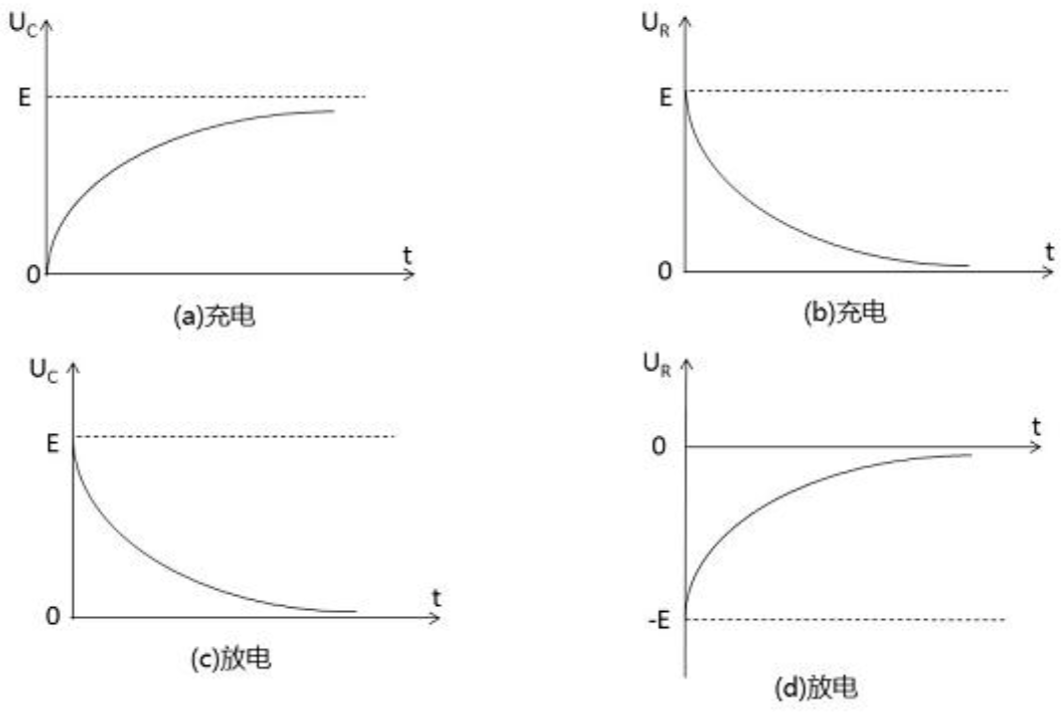
\includegraphics[width=0.7\textwidth]{fig2.png}
    \caption{}
\end{figure}

对于充电过程，由式(1)可知，当 $t=\tau$ 时，电容电压升至 $u_C=(1-1/e)E\approx 0.632E$；对于放电过程，由式(2)可知，当 $t=\tau$ 时，电容电压下降至 $u_C=E/e\approx 0.368E$。这样利用充电或放电曲线测出 $u_C=0.632E$ 或 $u_C=0.368E$ 所对应的时间就是时间常数 $\tau$，若 $R$ 已知，由 $\tau=RC$ 即可求出电容 $C$ 值。

在 Figure 1(a) 中，电容 $C$ 充电、放电的时间常数相同均为 $\tau=RC$ 。在 Figure 1(b) 中，电容 $C$ 充电时间常数为 $\tau_{充电}=R_1C$ ，放电时间常数 $\tau_{放}=R_2C$ 。如果 $\tau_{充}\gg \tau_{放}$ 或 $\tau_{充}\ll\tau_{放}$ ，这就是电子技术中利用 $u_c$ 产生锯齿波电压的基础。

\subsection{RL电路的暂态过程}
\begin{figure}[H]
    \centering
    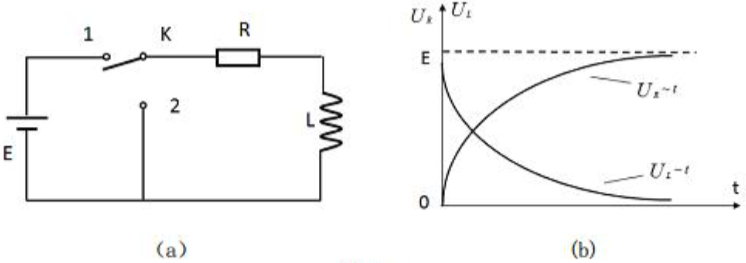
\includegraphics[width=0.7\textwidth]{fig3.png}
    \caption{}
\end{figure}

由电感 $L$ 和电阻 $R$ 串联的电路如 Figure 3(a) 所示。
当开关 $K$ 合至“1”时，电源接通，但由于电感中电流不能突变，所以电路中电流将逐渐增大，同时电感中储存的磁场能量也不断增加，直到暂态过程结束，电路达到稳态为止。
而当开关 $K$ 由“1”置“2”时，电感中储存的磁场能量通过 $R$ 进行释放，电路中的电流将逐渐衰减，直到其能量全部被电阻 $R$ 消耗掉为止。在这两种暂态过程中，$u_L$、$u_R$ 随时间 $t$ 的变化规律为：

充电电流增长过程
\begin{equation}
    \begin{cases}
        u_L=Ee^{-\frac{t}{\tau}}\\
        u_R=E(1-e^{-\frac{t}{\tau}})
    \end{cases}
\end{equation}

放电电流衰减过程
\begin{equation}
    \begin{cases}
        u_L=-Ee^{-\frac{t}\tau}\\
        u_R=Ee^{-\frac{t}{\tau}}
    \end{cases}
\end{equation}
上两式中的 $\tau=L/R$ ，为 RL 电路的时间常数，同 RC 电路一样，$\tau$ 越大，RL 电路的暂态过程越长。电路增长过程中 $u_L-t$、$u_R-t$ 的关系曲线如 Figure 3(b) 所示。

\subsection{RLC电路的暂态过程}
由电阻 $R$、电感 $L$、电容 $C$ 串联组成的电路如 Figure 4 所示。
先将开关 $K$ 置“1”，电源通过 $R$、$L$ 给电容 $C$ 充电，充电到 $u_C=E$ 后，再将 $K$ 由“1”置“2”位置，电容就在闭合的 RLC 电路中放电。
充、放电过程均为暂态过程。充、放电电路方程为：
\begin{equation}
    LC\frac{\mathrm d^2u_C}{\mathrm dt^2}+RC\frac{\mathrm du_C}{\mathrm dt}+u_C=\begin{cases}
        E&(充电)\\
        0&(放电)
    \end{cases}
\end{equation}
\begin{figure}[H]
    \centering
    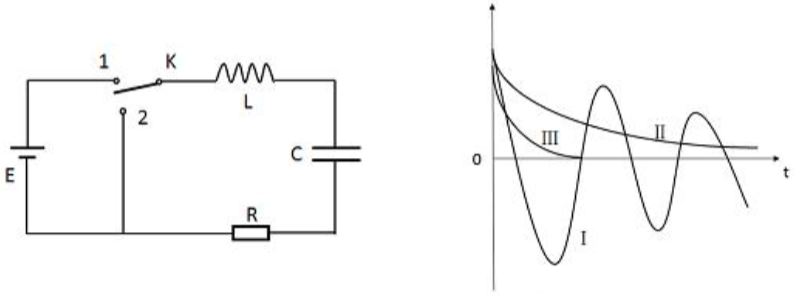
\includegraphics[width=0.7\textwidth]{fig4.png}
    \caption{}    
\end{figure}

对于放电过程：初始条件 $t=0$，$u_C=E$，$\frac{\mathrm du_C}{\mathrm dt}=0$。其解分为三种情况：

(1) $R^2<4L/C$
\begin{equation}
    u_C=\sqrt{\frac{4L}{4L-R^2C}}Ee^{-\alpha t}\cos(\omega t+\varphi)
\end{equation}
式中 $\alpha = \dfrac{R}{2L}$，$\omega = \dfrac{1}{\sqrt{LC}} \sqrt{1 - \dfrac{R^2 C}{4L}}$ 为衰减振荡的圆频率。
$u_C$ 随 $t$ 变化的规律如 Figure 4 中曲线Ⅰ所示。由图可以看出，随着时间 $t$ 增长，$u_C$ 以衰减振荡的方式逐渐衰减至零。这种衰减振荡的放电过程也叫做欠阻尼状态。

(2) $R^2>4L/C$
\begin{equation}
    u_C=\sqrt{\frac{4L}{R^2C-4L}}Ee^{-\omega t}\mathrm{sh}(\beta t+\varphi')
\end{equation}
式中 $\beta = \dfrac{1}{\sqrt{LC}} \sqrt{\dfrac{R^2 C}{4L} - 1}$。$u_C$ 随时间 $t$ 的变化规律如 Figure 4 中曲线Ⅱ所示，它以缓慢的方式逐渐衰减至零。此过程为非振荡放电过程，也叫做过阻尼状态。

(3) $R^2=4L/C$
\begin{equation}
    u_C=E(1+\alpha t)e^{-\omega t}
\end{equation}
$u_C$ 随时间 $t$ 的变化规律如 Figure 4 中曲线Ⅲ所示，仍属于非振荡放电类型，但正好是非振荡与振荡的分界线，故称为临界非振荡放电过程，也叫做临界阻尼状态。

通过上述分析可知，RLC 电路放电的暂态过程有三种情况，究竟属于哪一种取决于电路中元件的参数。放电过程以临界非振荡方式趋于平衡位置为最快。

对于 RLC 电路的充电过程，初始条件为 $t=0$，$u_C=0$，$\dfrac{\mathrm du_C}{\mathrm dt}=0$。类似上述分析，电容$C$上充电电压$u_C$随时间$t$的变化规律也有下面三种情况：


(1) $R^2 < 4L/C$
\begin{equation}
    u_C = E\left[1 - \sqrt{\frac{4L}{4L - R^2 C}} \mathrm{e}^{-\alpha t} \cos(\omega t + \varphi)\right]
\end{equation}

(2) $R^2 > 4L/C$
\begin{equation}
u_C = E\left[1 - \sqrt{\frac{4L}{R^2 C - 4L}} \mathrm{e}^{-\alpha t} \mathrm{sh}(\beta t + \varphi')\right]
\end{equation}

(3) $R^2 = 4L/C$
\begin{equation}
u_C = E\left[1 - (1 + \alpha t)\mathrm{e}^{-\alpha t}\right] \tag{21.10}
\end{equation}

对应的充电曲线如图21.6所示。曲线Ⅰ为振荡充电过程，属于欠阻尼状态；曲线Ⅱ为非振荡充电过程，属于过阻尼状态；曲线Ⅲ为临界非振荡充电过程，属于临界阻尼状态，且在此状
态下 $u_C$ 趋于平衡位置最快。

\begin{figure}[H]
    \centering
    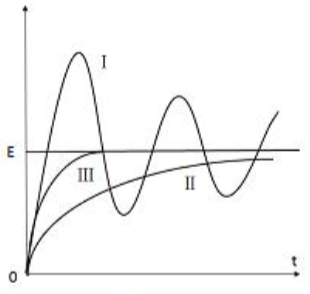
\includegraphics[width=0.35\textwidth]{fig5.png}
    \caption{}
\end{figure}

\section{仪器用具}
LTspice 软件模拟：示波器、方波信号发生器、标准电容($0.1\mathrm{\mu F}$)，标准电感($0.1\mathrm H$)，电阻等。

\section{实验内容}

\subsection{观察 RC 电路的暂态过程}
(1) 观察 $u_C$ 波形。按 Figure 6 中的电路图联接线路。调节方波发生器的周期 $T$ 、输出幅度，显示出方波和电容 $C$ 的充、放电曲线波形。解释观察到的波形，改变 $R$ 的大小，分析观察到的现象。

\begin{figure}[H]
    \centering
    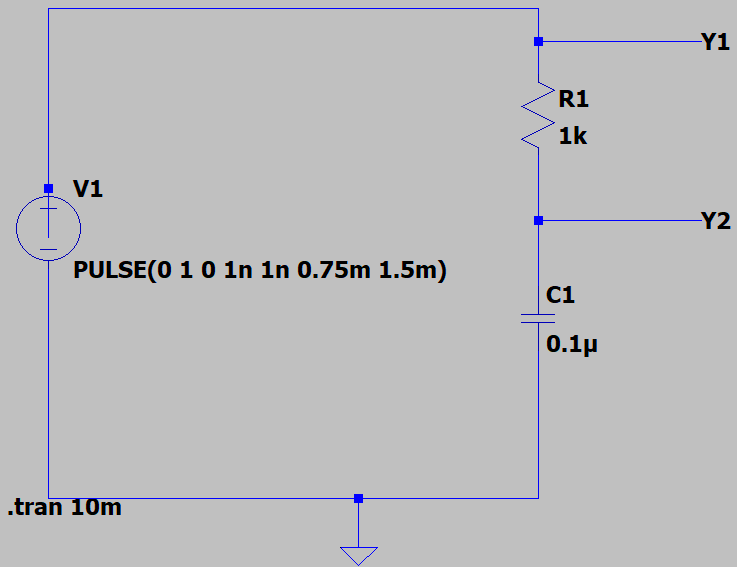
\includegraphics[width=0.5\textwidth]{fig6.png}
    \caption{}
\end{figure}

\begin{figure}[H]
    \centering
    \begin{subfigure}[b]{0.3\textwidth}
        \centering
        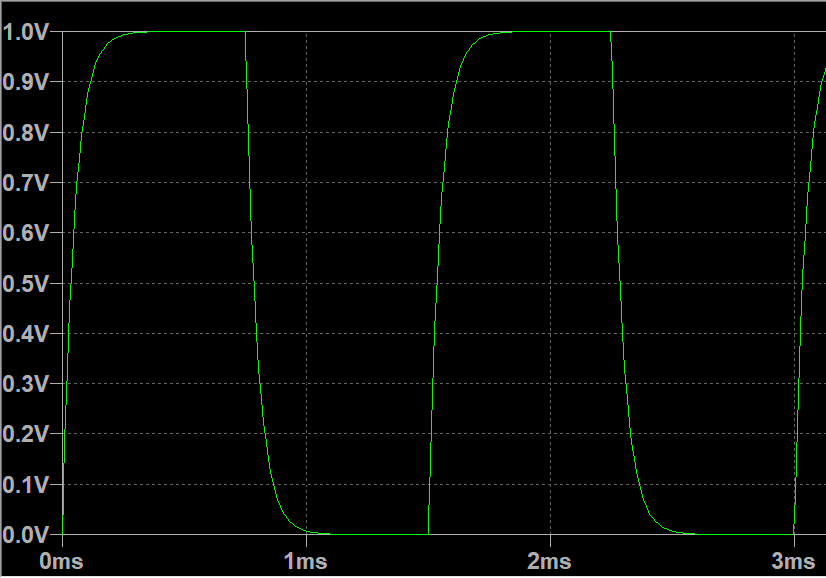
\includegraphics[width=\textwidth]{fig7a.png}
        \caption{$R=0.5k\Omega$}
    \end{subfigure}
    \hfil
    \begin{subfigure}[b]{0.3\textwidth}
        \centering
        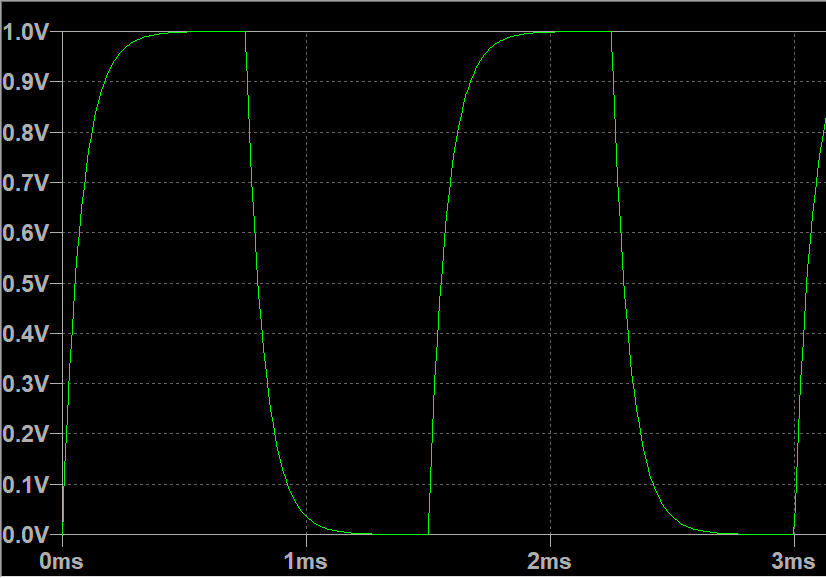
\includegraphics[width=\textwidth]{fig7c.png}
        \caption{$R=0.75k\Omega$}
    \end{subfigure}
    \hfil
    \begin{subfigure}[b]{0.3\textwidth}
        \centering
        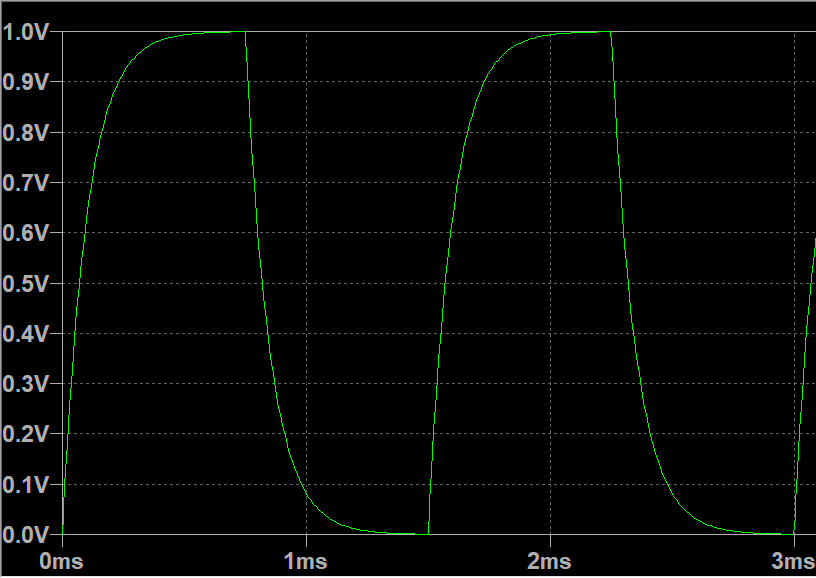
\includegraphics[width=\textwidth]{fig7b.png}
        \caption{$R=1k\Omega$}
    \end{subfigure}
    \caption{$u_C$ 波形}
\end{figure}

观察到 $u_C$ 先上升后下降，分别对应充电和放电过程。改变 $R$ 的值，发现充、放电随 $R$ 的增大而增大，原因是时间常数 $\tau=RC$ 增大。

(2) 测量 RC 电路的时间常数 $\tau$ 及电容。根据曲线测出该电路的时间常数 $\tau$ ，并与理论值比较。同时由 $\tau$ 可求出电容 $C$ 值（$R$ 已知）.

\begin{table}[H]
    \centering    
    \caption{时间常数 $\tau$ 和电容 $C$ 测量}
    \begin{tabular}{cccc}
        \hline\hline
        $i$            & 1   & 2    & 3    \\
        $R_i/k\Omega$  & 0.5        & 0.75      & 1    \\
        $\tau_i/\mu s$ & 50.041186  &74.752883  & 100.57661          \\
        $C/\mu F$      & 1.000823   &0.996705           &  1.005766       \\  
        \hline\hline
    \end{tabular}
\end{table}

(3) 观察微分电路的微分脉冲。调节方波信号周期 $T$ 或 $R$ 值，同时调节示波器可使示波器显示出如 Figure 8 所示的 $u_R$ 波形。在此基础上改变 $R$ 值或方波周期 $T$ 观察 $u_R$ 波形有何变化，解释观察到的现象。

\begin{figure}[H]
    \centering
    \begin{subfigure}[b]{0.3\textwidth}
        \centering
        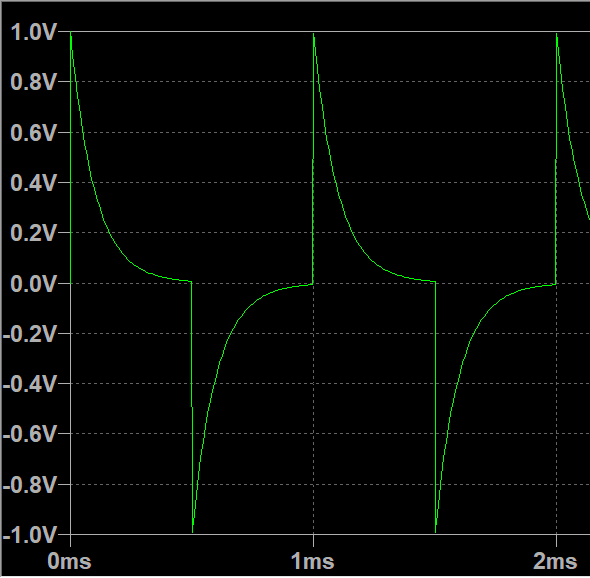
\includegraphics[width=\textwidth]{fig8a.png}
        \caption{$R=1k\Omega$,$T=1ms$}
    \end{subfigure}
    \hfil
    \begin{subfigure}[b]{0.3\textwidth}
        \centering
        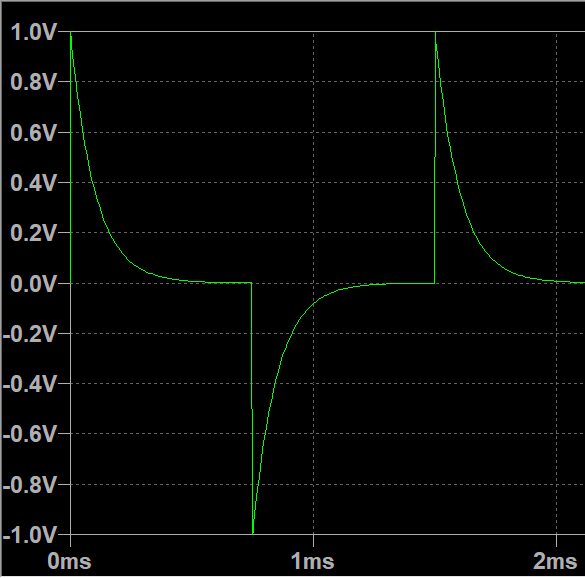
\includegraphics[width=\textwidth]{fig8b.png}
        \caption{$R=1k\Omega$,$T=1.5ms$}
    \end{subfigure}
    \hfil
    \begin{subfigure}[b]{0.3\textwidth}
        \centering
        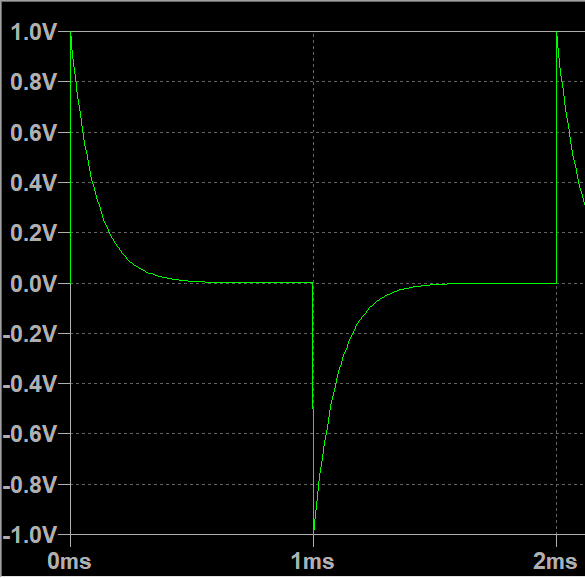
\includegraphics[width=\textwidth]{fig8c.png}
        \caption{$R=1k\Omega$,$T=2ms$}
    \end{subfigure}
    \vfil
    \begin{subfigure}[b]{0.3\textwidth}
        \centering
        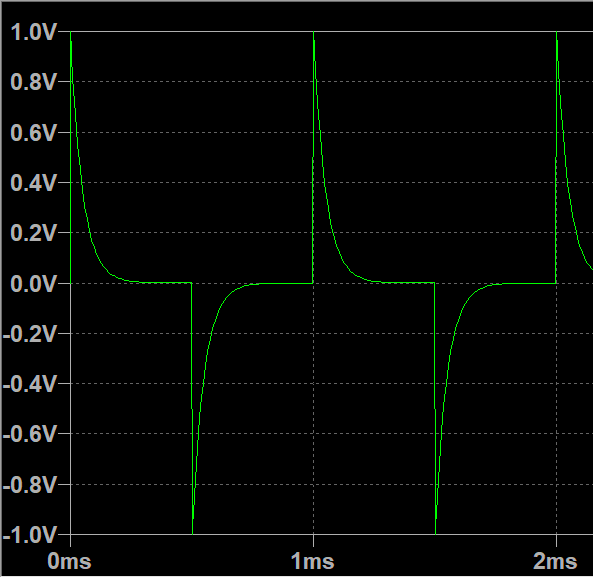
\includegraphics[width=\textwidth]{fig9a.png}
        \caption{$R=0.5k\Omega$,$T=1ms$}
    \end{subfigure}
    \hfil
    \begin{subfigure}[b]{0.3\textwidth}
        \centering
        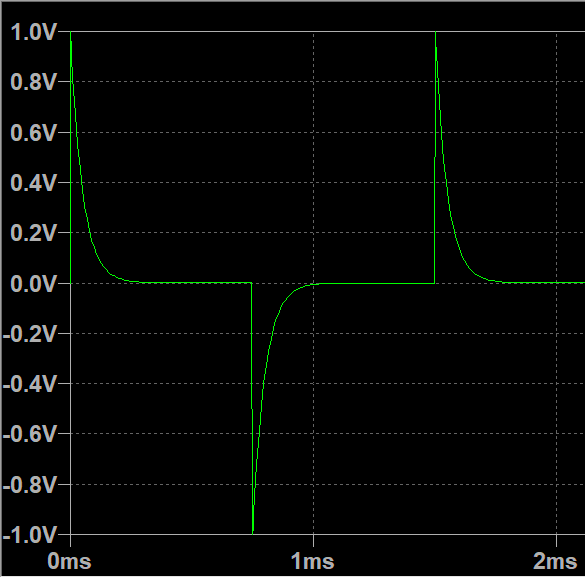
\includegraphics[width=\textwidth]{fig9b.png}
        \caption{$R=0.5k\Omega$,$T=1.5ms$}
    \end{subfigure}
    \hfil
    \begin{subfigure}[b]{0.3\textwidth}
        \centering
        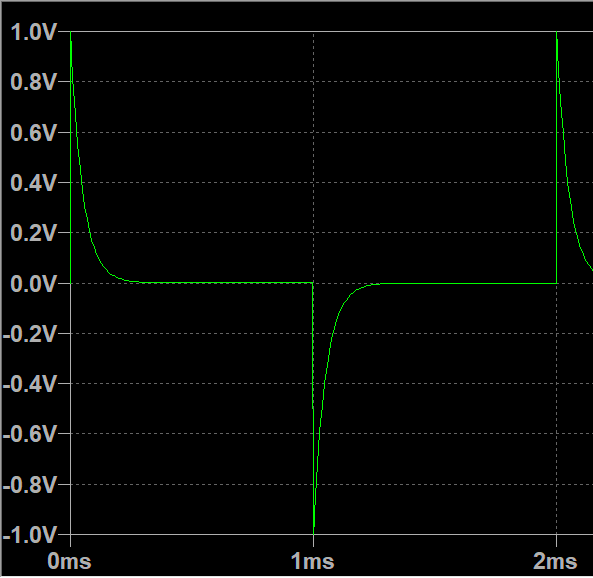
\includegraphics[width=\textwidth]{fig9c.png}
        \caption{$R=0.5k\Omega$,$T=2ms$}
    \end{subfigure}
    \caption{$u_C$ 波形}
\end{figure}

观察到，方波周期 $T$ 影响波形出现的频率，电阻 $R$ 值越低，波形越窄。

调节方波周期 $T$ 到足够大($T=5\sim10\tau$，即满足 $T\gg \tau=RC$)，同时适当调节 $R$ 值及示波器，在屏幕上可观察到如 Figure 9 所示的正负尖脉冲波形。这就是微分脉冲，该电路称为微分电路。 

\begin{figure}[H]
    \centering
    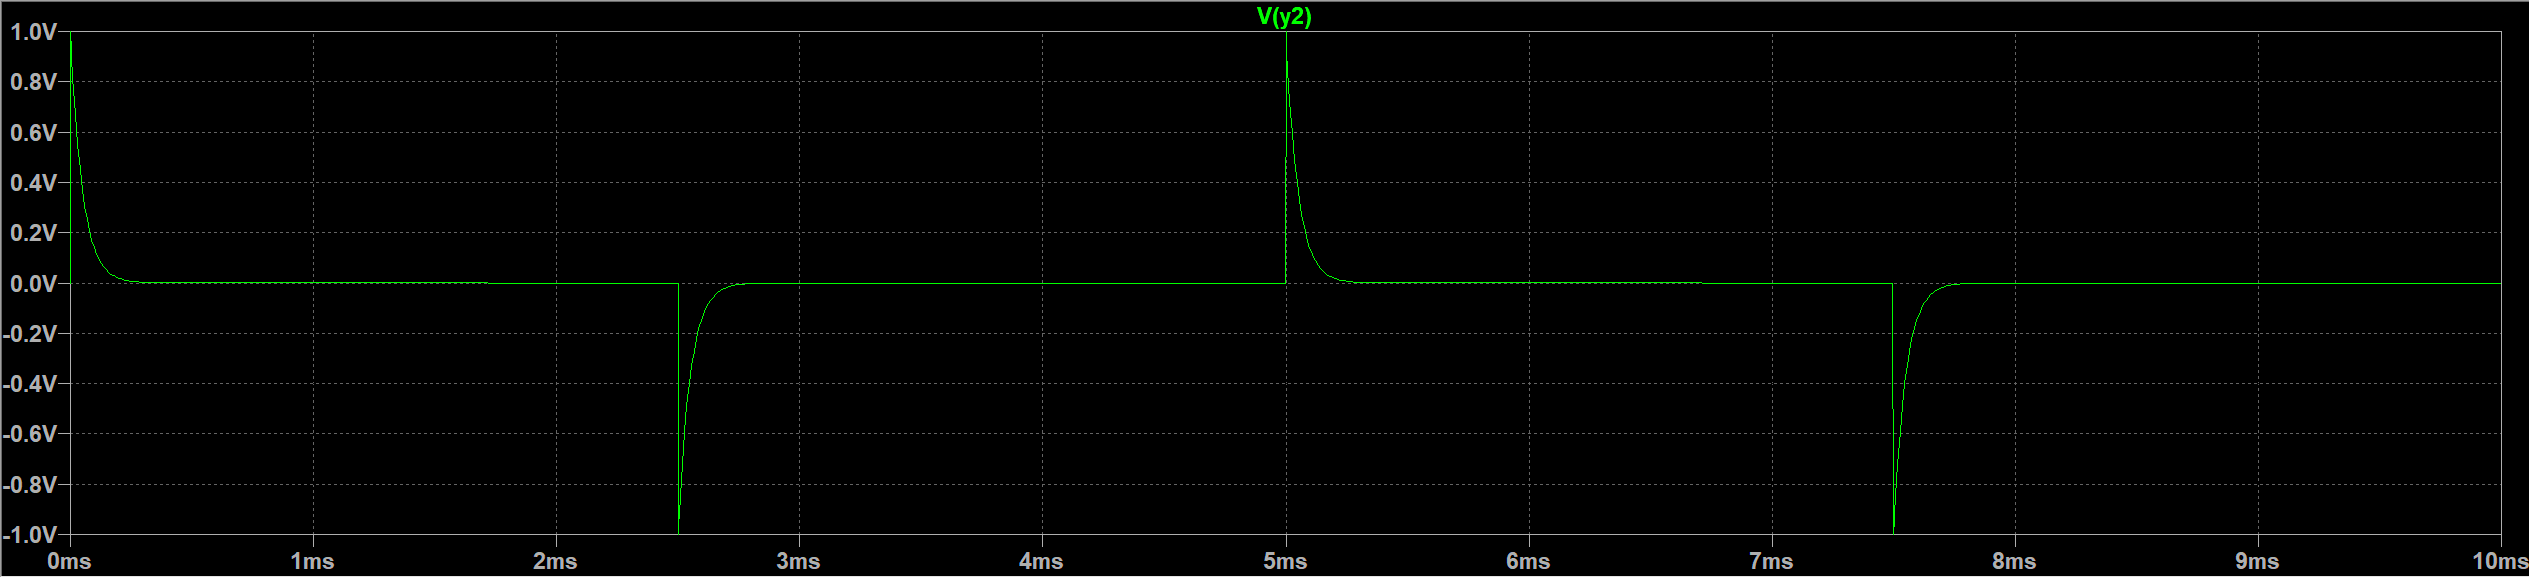
\includegraphics[width=\textwidth]{fig10.png}
    \caption{}
\end{figure}

\subsection{观察 RL 电路的暂态过程}
按 Figure 10(a) 联接线路，观察电感上电压 $u_L$ 在电流增长和衰减过程中的曲线波形，如 Figure 10(b) 所示。解释所观察到的图形。

\begin{figure}[H]
    \centering
    \begin{subfigure}[c]{0.45\textwidth}
        \centering
        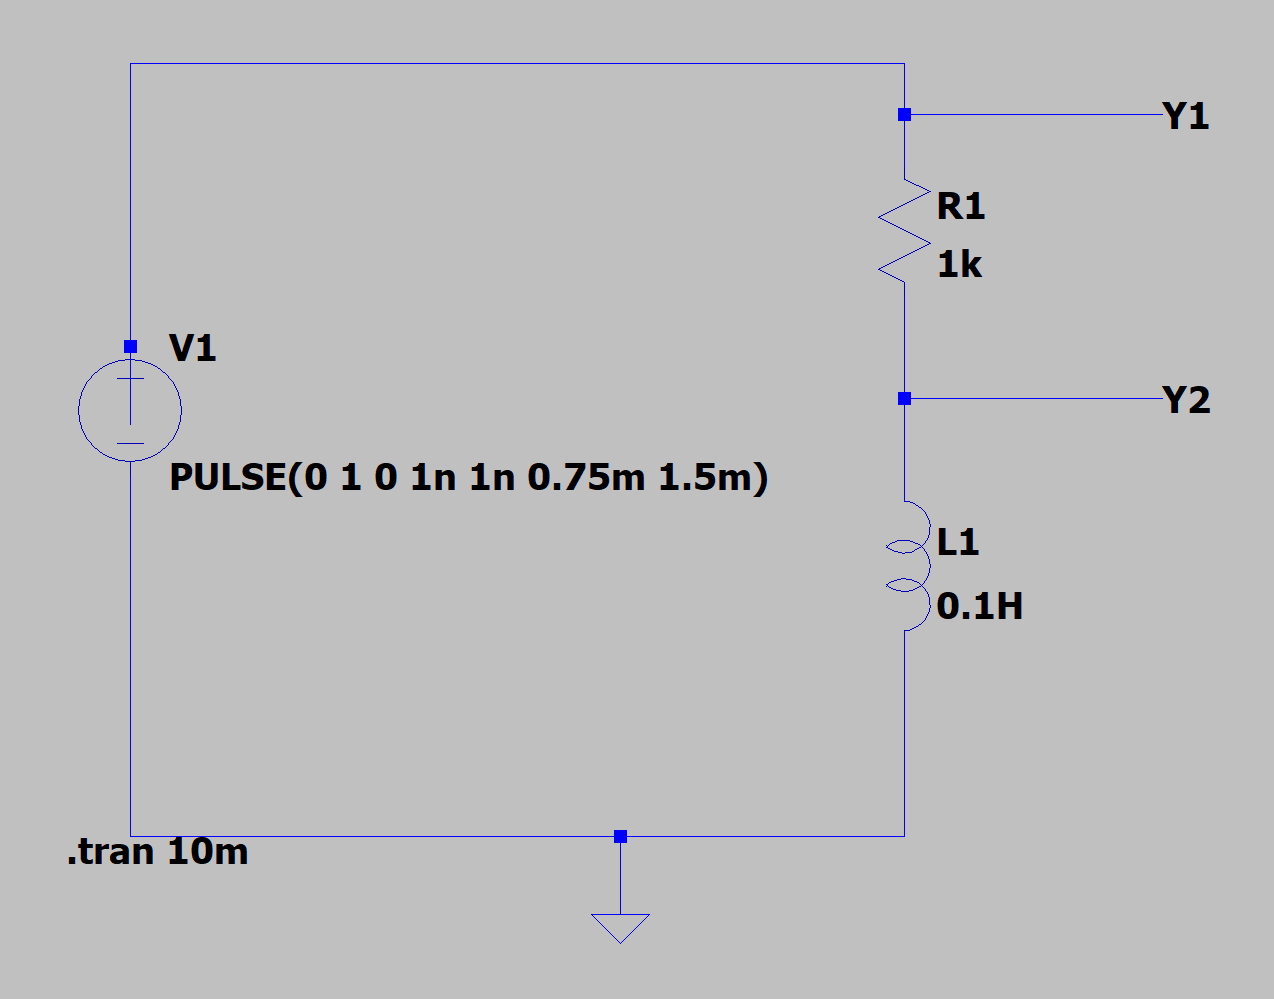
\includegraphics[width=\textwidth]{fig11.png}
        \caption{}
    \end{subfigure}
    \hfil
    \begin{subfigure}[c]{0.45\textwidth}
        \centering
        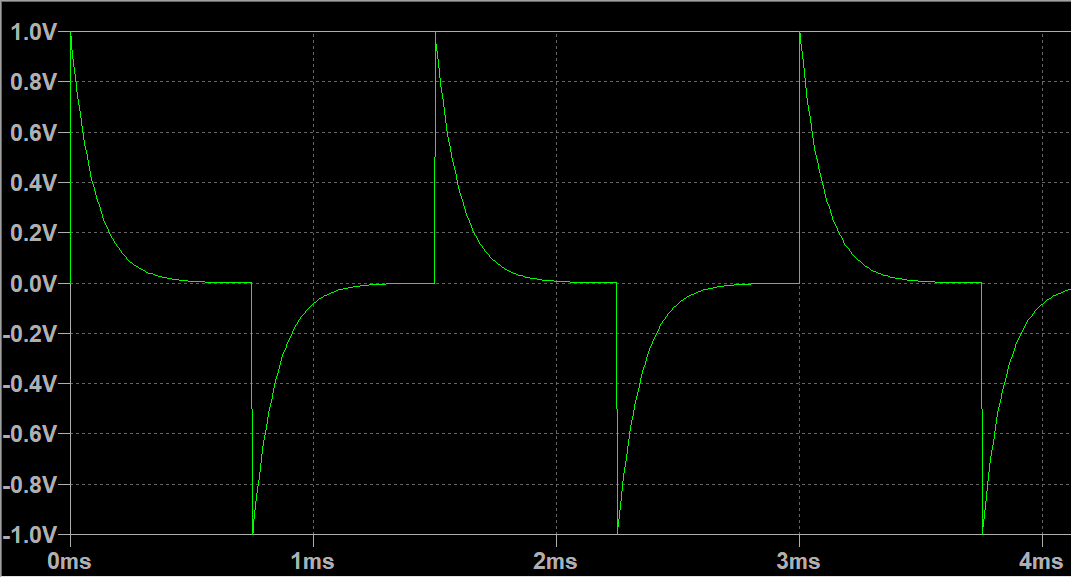
\includegraphics[width=\textwidth]{fig11b.png}
        \caption{}
    \end{subfigure}
    \caption{}
\end{figure}

充、放电时，电感阻碍电流变化。刚开始充电时，电流为 0 ，视为断路，两端电压 $u_L$ 等于电源电压，然后电压 $u_L$ 慢慢下降为零。放电时，电流方向相反，电压符号发生改变。

测出RL电路的时间常数$\tau$，并与理论值比较。若$R$已知由$\tau$可求出电感$L$值。

\begin{table}[H]
    \centering    
    \caption{时间常数 $\tau$ 和电容 $L$ 测量}
    \begin{tabular}{cccc}
        \hline\hline
        $\tau/\mu s$  &  $L/H$      \\
        99.217463  & 0.099217      \\
        \hline\hline
    \end{tabular}
\end{table}

\subsection{观察 RLC 电路的暂态过程}
联接线路如 Figure 11 所示。观察电容两端电压 $u_C$ 在充、放电过程中的变化规律。调节 $R$ 的大小，观察不同阻尼状态下的波形。

\begin{figure}[H]
    \centering
    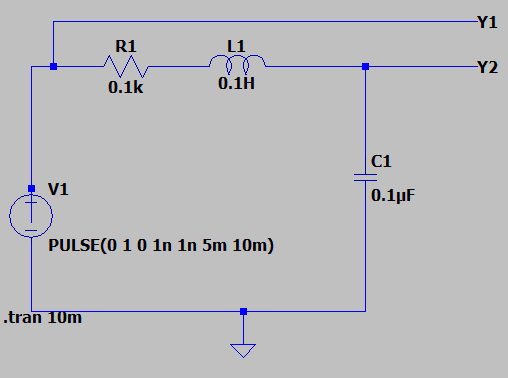
\includegraphics[width=0.6\textwidth]{fig12.png}
    \caption{}
\end{figure}

\begin{figure}[H]
    \centering
    \begin{subfigure}[c]{\textwidth}
        \centering
        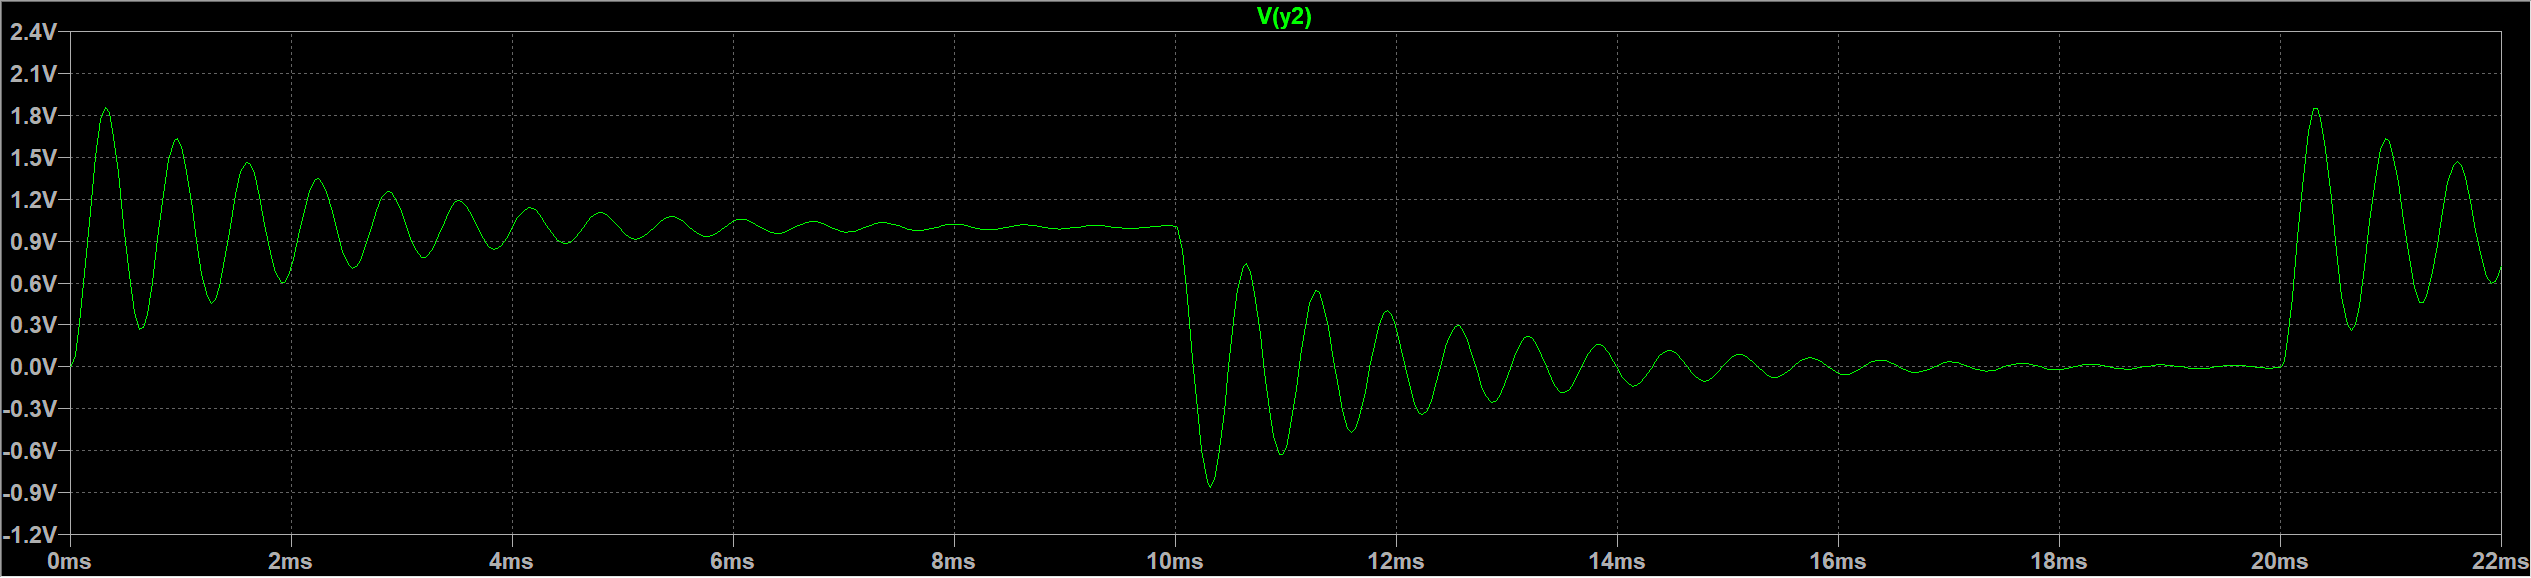
\includegraphics[width=\textwidth]{fig13a.png}
        \caption{欠阻尼状态 $R=0.1 K\Omega$}
    \end{subfigure}
    \vfil
    \begin{subfigure}[c]{\textwidth}
        \centering
        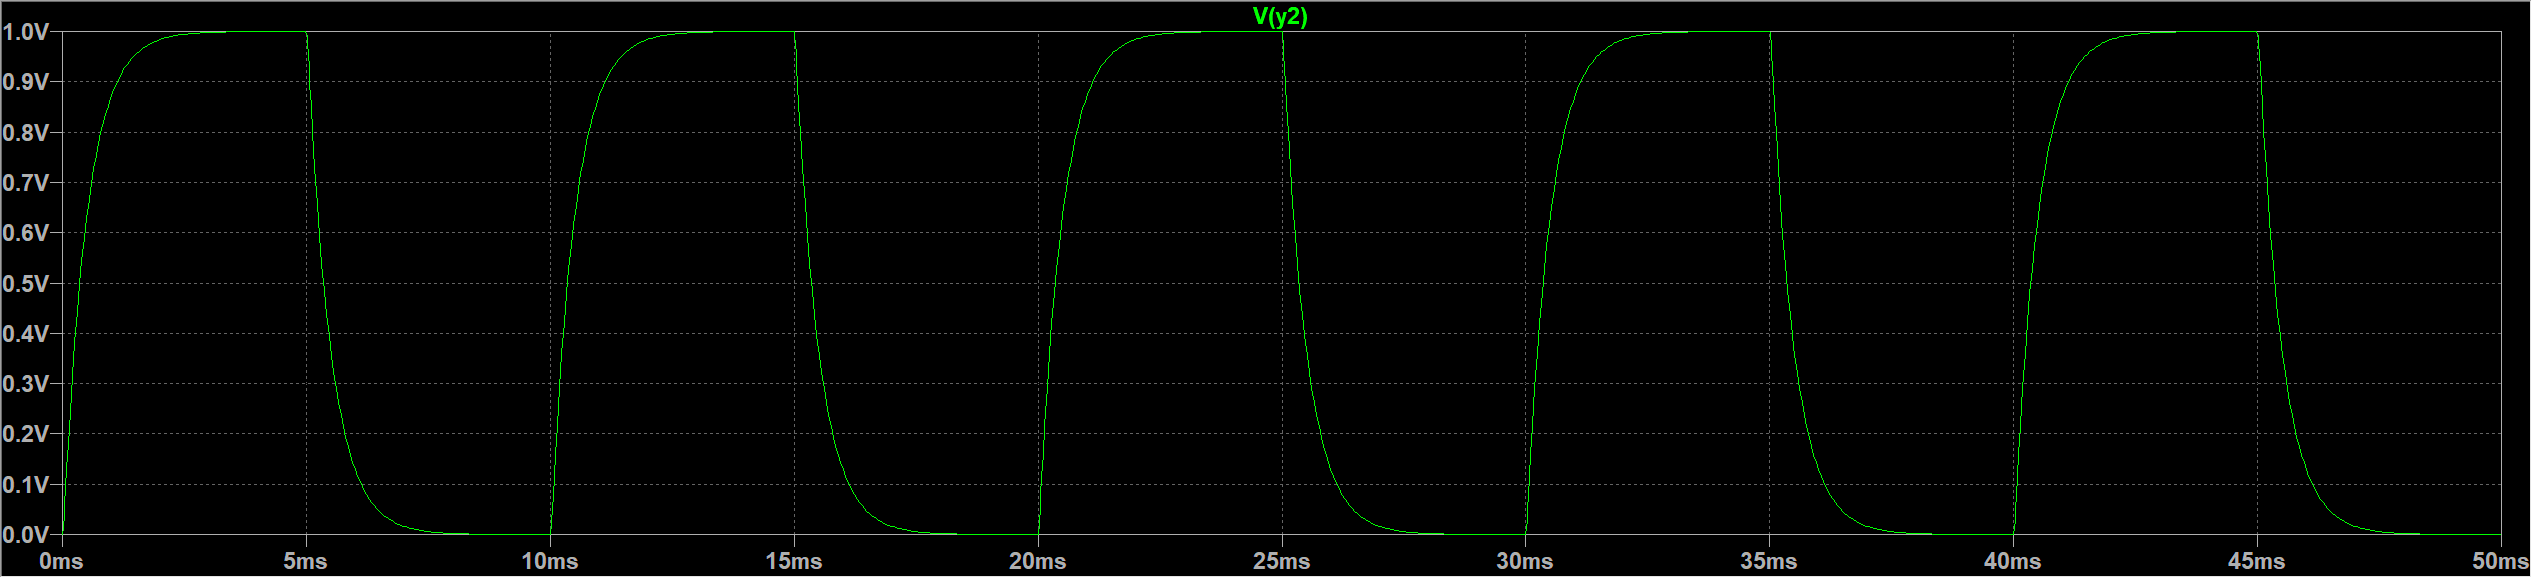
\includegraphics[width=\textwidth]{fig13b.png}
        \caption{过阻尼状态 $R=5 K\Omega$}
    \end{subfigure}
    \vfil
    \begin{subfigure}[c]{\textwidth}
        \centering
        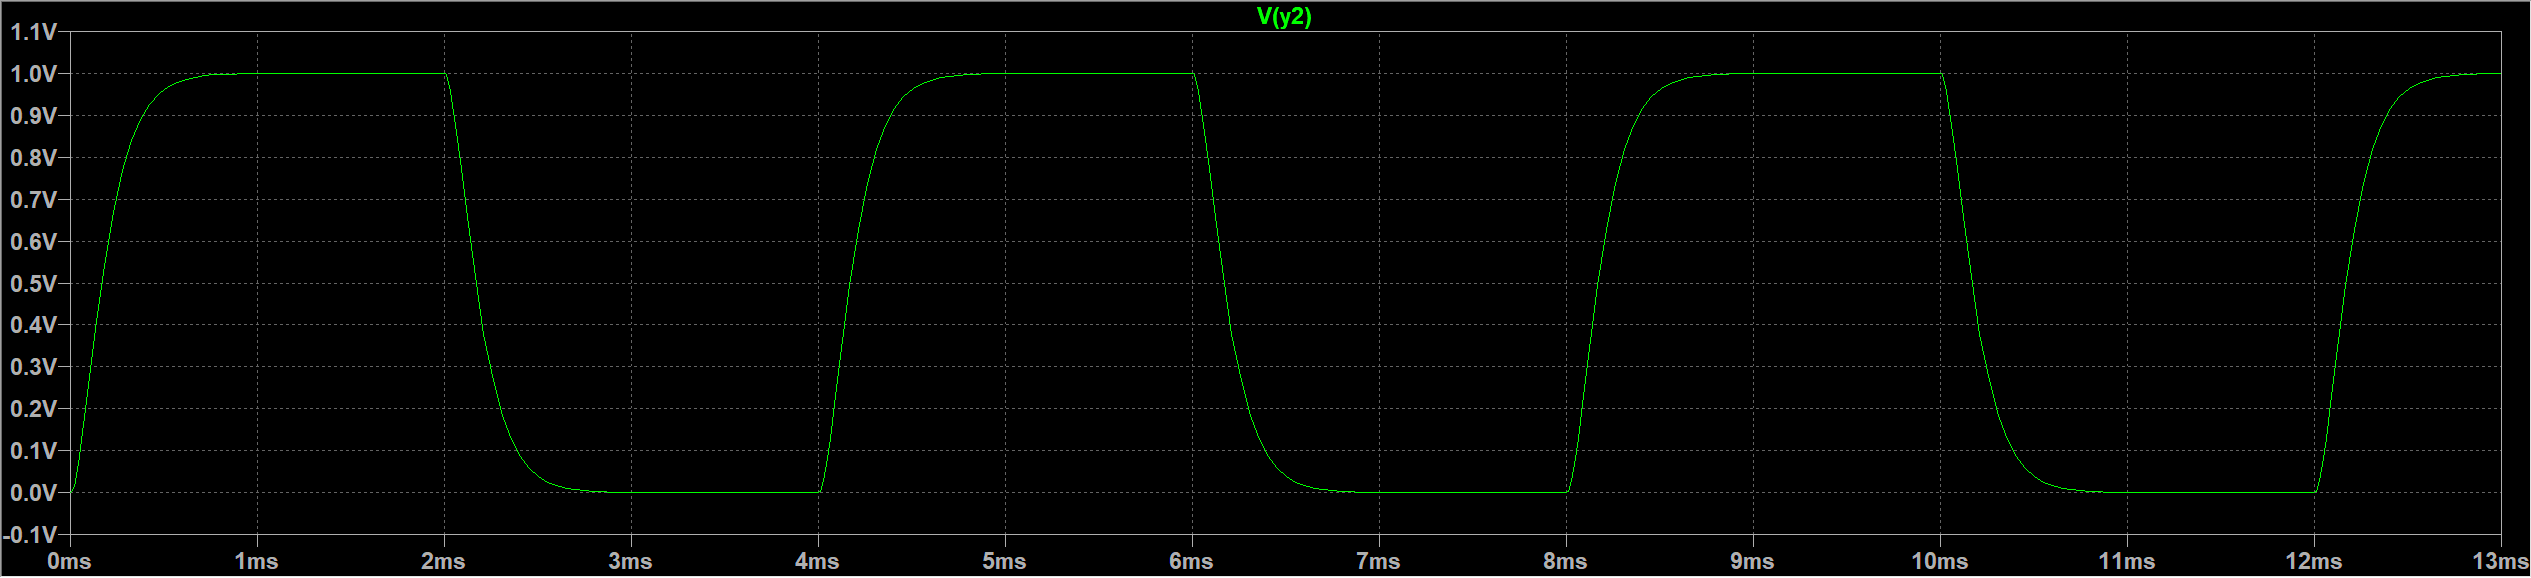
\includegraphics[width=\textwidth]{fig13c.png}
        \caption{临界阻尼状态 $R=2 K\Omega$}
    \end{subfigure}
    \caption{}
\end{figure}

\section{心得体会}
本实验通过 LTspice 仿真模拟，探究了 RC、RL、RLC 电路的暂态过程。既直观清晰地展现了不同电路对应的暂态过程，了解了 RC、RL 电路的时间常数，以及 RLC 电路的三种阻尼状态，还学习了 LTspice 的使用，为日后学习提供了不小的帮助。

\end{document}